\section{Security and Deniability}
The data stored in \gls{FFS} images is encrypted with state-of-the-art encryption standards. Using \gls{AES}-\gls{GCM}, \gls{FFS} does not only provide confidentiality of the data, but it also provides the authenticity of the data. The cryptographic algorithms are implemented using good cryptographic standards, such as cryptographic secure number generators\,\cite{RandomNumberGeneratorCryptoWiki2021}. However, the security of \gls{FFS} is dependent on, among other things, the password the user chooses. A bad password, for instance, short or commonly used, is easily breakable for an adversary. An adversary who has access to an \gls{FFS} encrypted image could brute-force the bad password used to derive the encryption key much faster than they could brute-force the encryption key. \gls{FFS} does not put any constraints on the password used - as long as it is at least one byte it is acceptable for \gls{FFS}. This puts the responsibility on the user for the choice of password constraints. 

FFS puts a lot of trust in the open-source library Crypto++\,\cite{CryptoLibraryFree}. Crypto++ provides cryptographic functions that \gls{FFS} uses for, among other things, deriving the encryption key, encrypting the data, and verifying the authentication tag. While there are no reported CVE security vulnerabilities as of writing\,cite{CryptoppSecurityVulnerabilities}, there may be vulnerabilities that have not yet been discovered or that have been found but not published in the CVE database. There is also a possibility that \gls{FFS} provides vulnerabilities, such as side channels, which could be exploited. \gls{FFS} is developed by a single author without a review from anyone else.

Anyone with access to Flickr.com can view and download the original images stored by \gls{FFS}, both registered users on Flickr, and anonymous visitors. An example of how the profile might look is shown in Figure~\ref{fig:flickr_profile}. The images found on the account present little information about the filesystem. For users unaware of \gls{FFS} who view the Flickr profile, they see different sizes of images with seemingly randomly generated pixel colors. However, for adversaries who know about the details of \gls{FFS}, more information can be retrieved. For instance, they could assume that the most recently uploaded image to Flickr is representing the inode table. However, as we assume the adversary does not have access to the decryption key, they cannot read the data of the image and thus cannot verify that this is indeed the inode table. The exact number of files and directories in \gls{FFS} cannot be known precisely without access to the content of the inode table. Even if the Flickr account has, for instance, 15 images stored, and we know that one represents the inode table and one represents the root directory, it is not possible to conclude if other images stores file data or directory data. The remaining 13 images in the example could represent:
\begin{itemize}
	\item one big single file split over 13 images, or
	\item one big single directory split over 13 images, or
	\item 13 different files, or
	\item 13 different directories, or
	\item 1 directory and 12 different files, or
	\item 13 copies of the same file, et cetera.
\end{itemize}
It is also not possible to know if an image stored on Flickr has been uploaded by \gls{FFS} or by the user manually to further diffuse the amount of data stored on the service. For instance, by encrypting random data using \gls{FFS}'s encoder and uploading the images to Flickr, but without saving the posts in the inode table or in a directory of \gls{FFS}, the images will look indistinguishable from the other images on Flickr. Only with access to the decrypted inode table can one know if the image is stored in \gls{FFS} or not. However, it is possible that Flickr could have logs about the uploaded images, and be able to distinguish images uploaded from the \gls{API} from the user interface. Future research could extend \gls{FFS} to post encrypted random data at random time intervals to automatically diffuse the knowledge about the images on the \gls{OWS}. This would mean that even Flickr would not be able to distinguish the uploaded data as it would all be uploaded from the same service. One drawback of storing images on Flickr that are not stored in \gls{FFS} is that it decreases the storage capacity of \gls{FFS}.

\begin{figure}[!ht]
	\begin{center}
	  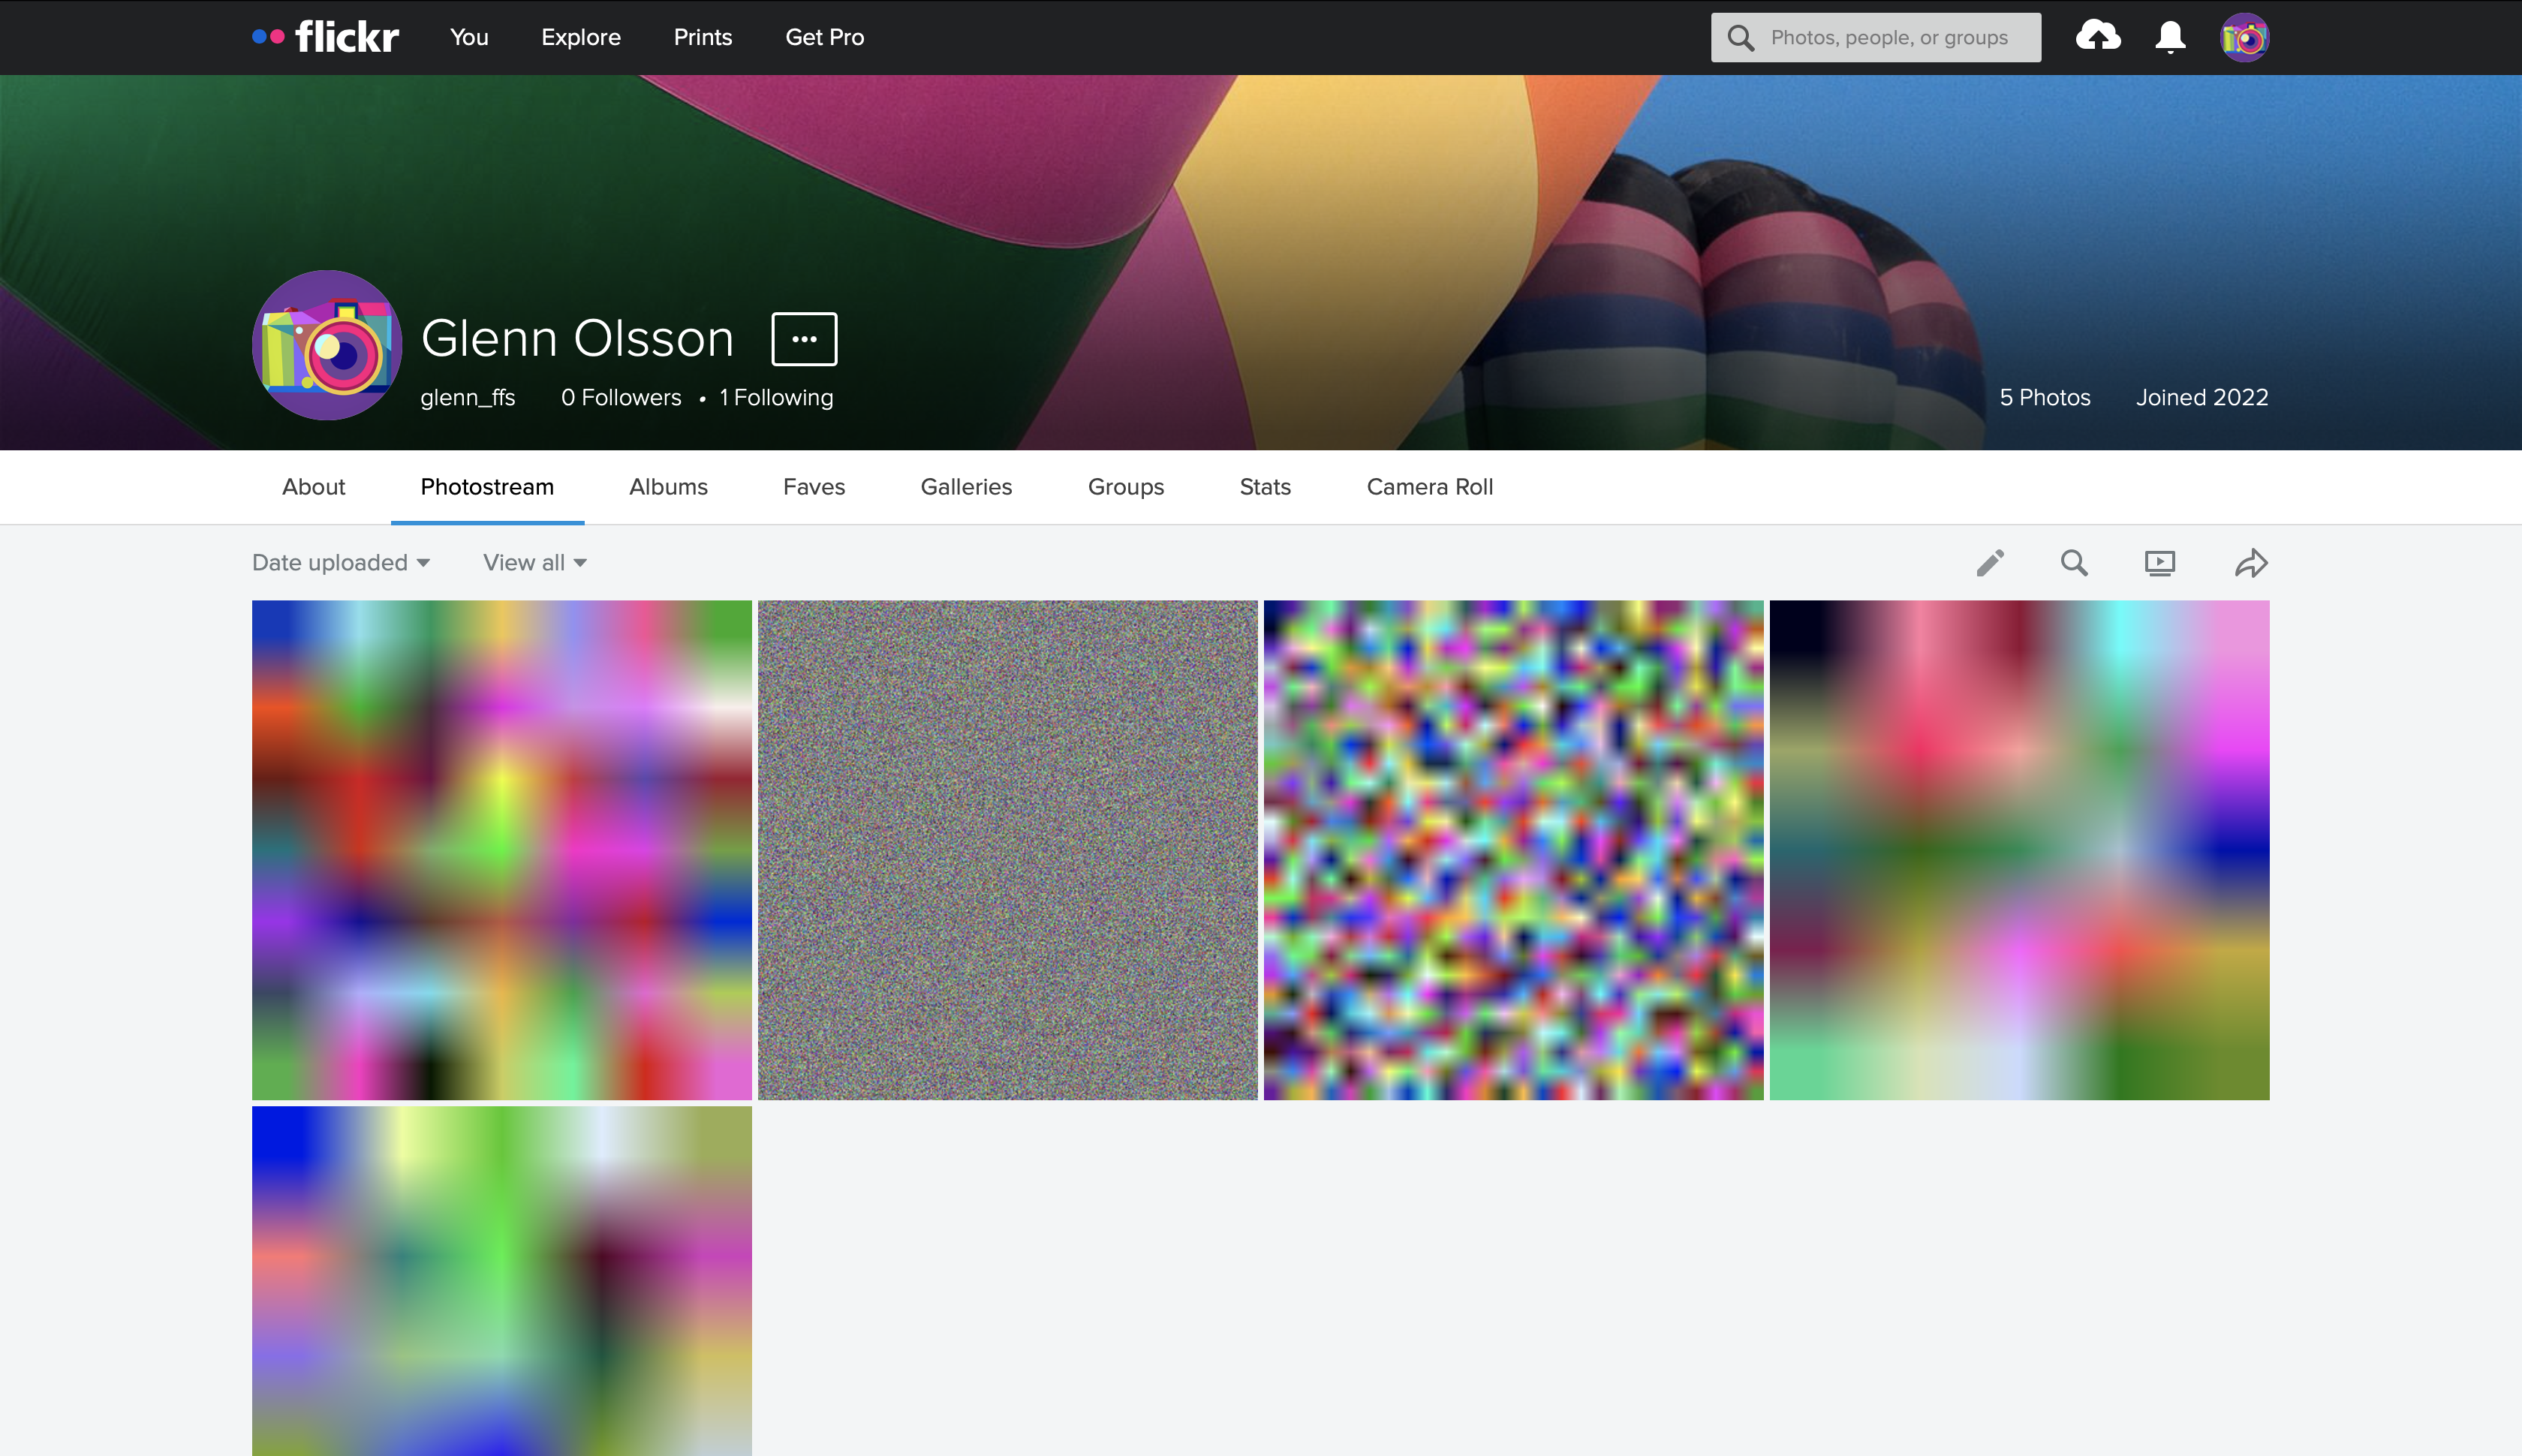
\includegraphics[width=0.8\textwidth]{figures/flickr_profile.png}
	\end{center}
	\caption[Screenshot of the Flickr profile used for \gls{FFS}]{Screenshot of the Flickr profile used for \gls{FFS}. At the moment of the screenshot, the filesystem is storing a previous version of this thesis in a directory inside the root directory. The images seen are the inode table, the thesis data, the root directory data, the subdirectory (containing the thesis) data, and a temporary file containing extra attributes of the thesis document created by macOS while \gls{FFS} was mounted (this file is sometimes referred to as a \textit{turd}\,\cite{geekosaurAnswerWhyAre2011}).}
	\label{fig:flickr_profile}
\end{figure}

The size of data stored in an image is not completely hidden. While the exact number of bytes of unencrypted data that the image stores is not possible to know without the decryption key, it is possible to get an estimate. If you know the binary structure of the image (as presented in Appendix~\ref{app:binary_rep}), you can find out how many bytes the encrypted cipher is, the value of the \gls{IV} data, the value of the salt used for the encryption key derivation, and the value of the authentication tag. By knowing the length of the cipher, the length of the unencrypted data can be placed in a range. The length of the cipher $L_c$ in bytes is divisible by 16 (as \gls{AES} is a 16-byte block cipher), and the length of the plain text must be less than $L_c$ due to the requirement of at least one bit of padding\,\cite{z.z.coderAnswerSizeData2010}. The smallest possible size for the length of the plain text is $L_c - 16$. Therefore, the length of the plain text $L_p$ is:
$$
	L_c - 16 \leq L_p < L_c
$$
By examining all the images stored on Flickr and their maximum possible value of $L_p$, it is possible to know the largest possible amount of data which is stored by \gls{FFS} on Flickr at a certain time. However, it is \textbf{not} possible to know if all this data is stored on \gls{FFS} through entries in the inode table. It is also \textbf{not} possible to know if the plain text represents a file or directory without the decrypted data of the inode table.

If a user supplies a different password when mounting \gls{FFS} than used previously, the images stored on Flickr cannot be decrypted. When \gls{FFS} tries to read the image it believes represents the inode table (the most recently uploaded image) and it fails, it will simply create a new inode table representing an empty filesystem, and upload the image representing this inode table, essentially replacing the potentially previous inode table (if it existed). As it is not possible to know if the images already uploaded to Flickr represent an inode table without the correct decryption key, it is impossible to determine if the image that could have represented the inode table was indeed an inode table encrypted with another password, or if it was some arbitrary data. In a potential rubber-hose situation\footnote{When an adversary might torture the user, with for instance a rubber hose. See Section~\ref{sec:rubber_hose}}, the user of the filesystem could easily claim that they uploaded \gls{FFS} images with arbitrary data, using randomly generated keys that they do not remember and that the filesystem is empty. There is no way to prove the existence of any meaningful data on Flickr without the decryption key. As the \gls{FFS} encoder also uses random salting for the encryption key, it is not even possible to prove that the images are encrypted with the same password as the encryption keys will differ for all images, even when the same password is used. 

As mentioned, we do however assume that an adversary has access to the structure of \gls{FFS} images as well. To counter this, the user who wants to hide its data could, after creating a filesystem containing meaningful information, mount \gls{FFS} again with another password. \gls{FFS} would then create a new inode table and upload this table, creating a dummy \gls{FFS}. In a rubber-hose situation, the user could give up the password to the dummy \gls{FFS} instance, which is empty. The adversary can verify that this password indeed decrypts the most recently uploaded image and that the unencrypted image data represents an empty inode table. If the user proceeds to claim that they do not know the passwords of the other images, the adversary cannot prove that they contain meaningful data nor that they have been uploaded by the user. These images could, for instance, have been uploaded by another user of \gls{FFS}. Further, with no password constraints by \gls{FFS}, a user could also create a dummy \gls{FFS} with a password that is easily breakable, to make the adversary believe they found the correct password if they perform a brute-force attack. As long as the user remembers which post represents the inode table, the images uploaded after this inode table could simply be removed from Flickr before mounting \gls{FFS} with the correct password when the user wants to access their actual \gls{FFS} instance. Alternatively, the user could save the image representing the inode table in another storage medium and upload it again when they want to access their actual \gls{FFS} instance.

One aspect where \gls{FFS} is better than \gls{GCSF} is its security against the potential adversary of the store owners. \gls{GCSF} stores the data in its original format on Google Drive, essentially providing an overlay filesystem for Google Drive. While this can be desired in certain situations, such as using \gls{GCSF} on one machine and the Google Drive website on another, it gives Google Drive access to your data. As mentioned, Google Drive encrypts your data from outside agents, but as they control the encryption and decryption keys themselves, the data stored can be accessed by the company. For instance, the data could be given to authorities who are requesting it with a subpoena. \gls{FFS} on the other hand gives the user control of all its data. While Flickr can give out the images uploaded by \gls{FFS}, this data can be accessed by anyone with access to Flickr.com anyway. A subpoena by authorities will not help more than possibly providing them with the IP addresses of origin of the uploaded content. The only way to access unencrypted data is by using the password that the user controls. This provides \gls{FFS} with one aspect of better security than \gls{GCSF}, but this might also be a factor why \gls{FFS} is slower than \gls{GCSF}. By requiring the data to be encrypted when it is written and uploaded, and decrypted when it is downloaded and read, \gls{FFS} will need to compute new cryptographic variables every time a file or directory is written which requires a lot of computations. Further, every time an image is read it must be decrypted, even if it is in the cache of \gls{FFS}. Decrypting an image requires a lot of computations as well as, other than decrypting the data, the decryption key must first be derived from the password. Meanwhile, it is possible that Google Drive is caching the unencrypted files, or performing the cryptographic computations on high-performance computers requiring less computation time. So while gaining a security aspect of the filesystem, \gls{FFS} sacrifices the performance of the filesystem operations.